\documentclass{article}
\usepackage{graphicx, tikz-cd, float} % Required for inserting images
\usepackage{amsmath, amssymb, amsthm, amsfonts, siunitx, physics, gensymb}
\AtBeginDocument{\RenewCommandCopy\qty\SI}
\usepackage[version=4]{mhchem}
\usepackage[most,many,breakable]{tcolorbox}
\usepackage{xcolor, fancyhdr, varwidth}
\usepackage[Glenn]{fncychap}
%Options: Sonny, Lenny, Glenn, Conny, Rejne, Bjarne, Bjornstrup
\usepackage{hyperref, cleveref}
\usepackage{icomma, enumitem} %comma as decimal and continue enumerate with [resume]
%%%%%%%%%%%%%%%%%%%%%%%%%%%%%%
% SELF MADE COLORS
%%%%%%%%%%%%%%%%%%%%%%%%%%%%%%
\definecolor{myg}{RGB}{56, 140, 70}
\definecolor{myb}{RGB}{45, 111, 177}
\definecolor{myr}{RGB}{199, 68, 64}
\definecolor{mytheorembg}{HTML}{F2F2F9}
\definecolor{mytheoremfr}{HTML}{00007B}
\definecolor{mylenmabg}{HTML}{FFFAF8}
\definecolor{mylenmafr}{HTML}{983b0f}
\definecolor{mypropbg}{HTML}{f2fbfc}
\definecolor{mypropfr}{HTML}{191971}
\definecolor{myexamplebg}{HTML}{F2FBF8}
\definecolor{myexamplefr}{HTML}{88D6D1}
\definecolor{myexampleti}{HTML}{2A7F7F}
\definecolor{mydefinitbg}{HTML}{E5E5FF}
\definecolor{mydefinitfr}{HTML}{3F3FA3}
\definecolor{notesgreen}{RGB}{0,162,0}
\definecolor{myp}{RGB}{197, 92, 212}
\definecolor{mygr}{HTML}{2C3338}
\definecolor{myred}{RGB}{127,0,0}
\definecolor{myyellow}{RGB}{169,121,69}
\definecolor{myexercisebg}{HTML}{F2FBF8}
\definecolor{myexercisefg}{HTML}{88D6D1}
%%%%%%%%%%%%%%%%%%%%%%%%%%%%%%%%%%%%%%%%%%%%%%%%%%%%%%%%%%%%%%%%%%%%%%
% Box environments for theorems and problems
%%%%%%%%%%%%%%%%%%%%%%%%%%%%%%%%%%%%%%%%%%%%%%%%%%%%%%%%%%%%%%%%%%%%%
\setlength{\parindent}{1cm}
%================================
% Question BOX
%================================
\makeatletter
\newtcbtheorem{question}{Opgave}{enhanced,
	breakable,
	colback=white,
	colframe=myb!80!black,
	attach boxed title to top left={yshift*=-\tcboxedtitleheight},
	fonttitle=\bfseries,
	title={#2},
	boxed title size=title,
	boxed title style={%
			sharp corners,
			rounded corners=northwest,
			colback=tcbcolframe,
			boxrule=0pt,
		},
	underlay boxed title={%
			\path[fill=tcbcolframe] (title.south west)--(title.south east)
			to[out=0, in=180] ([xshift=5mm]title.east)--
			(title.center-|frame.east)
			[rounded corners=\kvtcb@arc] |-
			(frame.north) -| cycle;
		},
	#1
}{def}
\makeatother
%================================
% DEFINITION BOX
%================================

\newtcbtheorem[]{Definition}{Definition}{enhanced,
	before skip=2mm,after skip=2mm, colback=red!5,colframe=red!80!black,boxrule=0.5mm,
	attach boxed title to top left={xshift=1cm,yshift*=1mm-\tcboxedtitleheight}, varwidth boxed title*=-3cm,
	boxed title style={frame code={
					\path[fill=tcbcolback]
					([yshift=-1mm,xshift=-1mm]frame.north west)
					arc[start angle=0,end angle=180,radius=1mm]
					([yshift=-1mm,xshift=1mm]frame.north east)
					arc[start angle=180,end angle=0,radius=1mm];
					\path[left color=tcbcolback!60!black,right color=tcbcolback!60!black,
						middle color=tcbcolback!80!black]
					([xshift=-2mm]frame.north west) -- ([xshift=2mm]frame.north east)
					[rounded corners=1mm]-- ([xshift=1mm,yshift=-1mm]frame.north east)
					-- (frame.south east) -- (frame.south west)
					-- ([xshift=-1mm,yshift=-1mm]frame.north west)
					[sharp corners]-- cycle;
				},interior engine=empty,
		},
	fonttitle=\bfseries,
	title={#2},#1}{def}
\newtcbtheorem[]{definition}{Definition}{enhanced,
	before skip=2mm,after skip=2mm, colback=red!5,colframe=red!80!black,boxrule=0.5mm,
	attach boxed title to top left={xshift=1cm,yshift*=1mm-\tcboxedtitleheight}, varwidth boxed title*=-3cm,
	boxed title style={frame code={
					\path[fill=tcbcolback]
					([yshift=-1mm,xshift=-1mm]frame.north west)
					arc[start angle=0,end angle=180,radius=1mm]
					([yshift=-1mm,xshift=1mm]frame.north east)
					arc[start angle=180,end angle=0,radius=1mm];
					\path[left color=tcbcolback!60!black,right color=tcbcolback!60!black,
						middle color=tcbcolback!80!black]
					([xshift=-2mm]frame.north west) -- ([xshift=2mm]frame.north east)
					[rounded corners=1mm]-- ([xshift=1mm,yshift=-1mm]frame.north east)
					-- (frame.south east) -- (frame.south west)
					-- ([xshift=-1mm,yshift=-1mm]frame.north west)
					[sharp corners]-- cycle;
				},interior engine=empty,
		},
	fonttitle=\bfseries,
	title={#2},#1}{def}

\newtcbtheorem{theo}%
    {Theorem}{}{theorem}
\newtcolorbox{prob}[1]{colback=red!5!white,colframe=red!50!black,fonttitle=\bfseries,title={#1}}
%================================
% NOTE BOX
%================================

\usetikzlibrary{arrows,calc,shadows.blur}
\tcbuselibrary{skins}
\newtcolorbox{note}[1][]{%
	enhanced jigsaw,
	colback=gray!20!white,%
	colframe=gray!80!black,
	size=small,
	boxrule=1pt,
	title=\textbf{Note:},
	halign title=flush center,
	coltitle=black,
	breakable,
	drop shadow=black!50!white,
	attach boxed title to top left={xshift=1cm,yshift=-\tcboxedtitleheight/2,yshifttext=-\tcboxedtitleheight/2},
	minipage boxed title=1.5cm,
	boxed title style={%
			colback=white,
			size=fbox,
			boxrule=1pt,
			boxsep=2pt,
			underlay={%
					\coordinate (dotA) at ($(interior.west) + (-0.5pt,0)$);
					\coordinate (dotB) at ($(interior.east) + (0.5pt,0)$);
					\begin{scope}
						\clip (interior.north west) rectangle ([xshift=3ex]interior.east);
						\filldraw [white, blur shadow={shadow opacity=60, shadow yshift=-.75ex}, rounded corners=2pt] (interior.north west) rectangle (interior.south east);
					\end{scope}
					\begin{scope}[gray!80!black]
						\fill (dotA) circle (2pt);
						\fill (dotB) circle (2pt);
					\end{scope}
				},
		},
	#1,
}

%%%%%%%%%%%%%%%%%%%%%%%%%%%%%%%%%%%%%%%%%%%%%%%%%%%%%%%%%%%%%%%%%
% SELF MADE COMMANDS
%%%%%%%%%%%%%%%%%%%%%%%%%%%%%%
\newcommand{\sol}{\setlength{\parindent}{0cm}\textbf{\textit{Løsning:}}\setlength{\parindent}{1cm}}
%%%%%%%%%%%%%%%%%%%%%%%%%%%%%%%%%
\usepackage[tmargin=2cm,rmargin=1in,lmargin=1in,margin=0.85in,bmargin=2cm,footskip=.2in]{geometry}\pagestyle{fancy}
\lhead{Minrui Kevin Zhou 2.b}
\rhead{Matematikaflevering 18}

\title{Aflevering 18\\
{\Large \textbf{2.b mat A}}}
\author{Kevin Zhou}
\date{November 2023}

\begin{document}
\maketitle
\section*{Bedømmelseskriterier:}
\begin{itemize}
    \setlength\itemsep{3cm}
    \Large
    \item  Redegørelse og dokumentation for metode
    \item Figurer, grafer og andre illustrationer
    \item Notation og layout
    \item Formidling og forklaring
\end{itemize}
\pagebreak

\begin{question}{}{}
  Funktionen $f:[0;6]\to \mathbb{R}$ er givet ved
  \[
  f(x)= x^3 -9x^2 +15x+5
  \] 
  \begin{itemize}
    \item[a.] Bestem monotoniforholdene for $f$.
    \item[b.] Bestem ekstrema for $f$.
    \item[c.] Tegn grafen for $f$.
  \end{itemize}
\end{question}
\sol \\ 
\textbf{a.} $f$ differentieres.
\[
\dv{f}{x}= 3x^2-18x+15 
\] 
Herefter finder vi de $x$-værdier, hvor $\dv{f}{x}=0$.
\begin{equation*}
  3x^2-18x+15=0 \implies x=1 \lor x=5
\end{equation*}
Vi ved, at $f'(x)$ har konstant fortegn i intervallerne $[0;1[, ]1;5[, ]5;6]$, da $f'(x)$ er kontinuert. 
Siden 
\begin{equation*}
\begin{split}
  f'(0)&=15\\
  f'(2)&=-9\\
  f'(6)&=15
\end{split}
\end{equation*}
så må følgende gælde med hensyn til monotoniforholdene for $f$.
\begin{equation*}
\begin{split}
  &f \text{ er voksende på } [0;1]\\
&f \text{ er aftagende på } [1;5]\\
&f \text{ er voksende på } [5;6]
\end{split}
\end{equation*}
\textbf{b.} Ekstremumsstederne for $f$ må være $0,1,5\;\text{og}\;6$, hvilket fremgår af \textbf{a.} 
Ekstrema for $f$ kan da nu udregnes.
\begin{equation*}
\begin{split}
  f(0)&= 5\\
  f(1)&= 12\\
  f(5)&= -20\\
  f(6)&= -13\\
\end{split}
\end{equation*}
\textbf{c.} I \cref{fig:1} ses grafen for $f$.
\begin{figure}[H]
\begin{center}
  \includegraphics[scale=0.2]{mat18_1.png}
\end{center}
\caption{Grafen for $f$ tegnet i GeoGebra}
\label{fig:1}
\end{figure}

\begin{question}{}{}
   Funktionen $f:\mathbb{R} \to \mathbb{R}$ er givet ved
  \[
  f(x)= x^3 \cdot e^x
  \] 
  \begin{itemize}
    \item[a.] Bestem minimum for $f$.
    \item[b.] Bestem en ligning for tangenten til grafen for $f$ i punktet $\left(1,f(1)\right)$.
    \item[c.] Tegn grafen for $f$.
  \end{itemize}
\end{question}
\sol \\ 
\textbf{a.} Funktionen differentieres med produktreglen.
\[
\dv{f}{x}=3x^2\cdot e^x + x^3\cdot e^x
\] 
Ekstremumsstederne findes ved at sætte lig med 0.
\[
3x^2\cdot e^x + x^3\cdot e^x=0 \implies x=-3 \lor x=0
\] 
Siden $f'(-1)>0$ og $-1 \in ]-3;0[$, er $f$ voksende i intervallet $[-3;0]$, så $-3$ er altså ekstremumssted til et minimum, der nu kan regnes.
\[
f(-3)=(-3)^3\cdot e^{-3}\approx -1,34 
\] 
\textbf{b.} Følgende må gælde for tangenten til grafen for $f$ i punktet $\left(1,f(1)\right)$.
\begin{equation*}
\begin{split}
  y&=f'(1)\cdot (x-1)+f(1)\\ 
  &= 4e^x\cdot (x-1) + e^x\\ 
  &= 4x\cdot e^x -3e^x
\end{split}
\end{equation*}
Altså er ligningen for tangenten $y=4x\cdot e^x -3e^x$.\\[1ex]
\textbf{c.} I \cref{fig:2} ses grafen for $f$.
\begin{figure}[H]
\begin{center}
  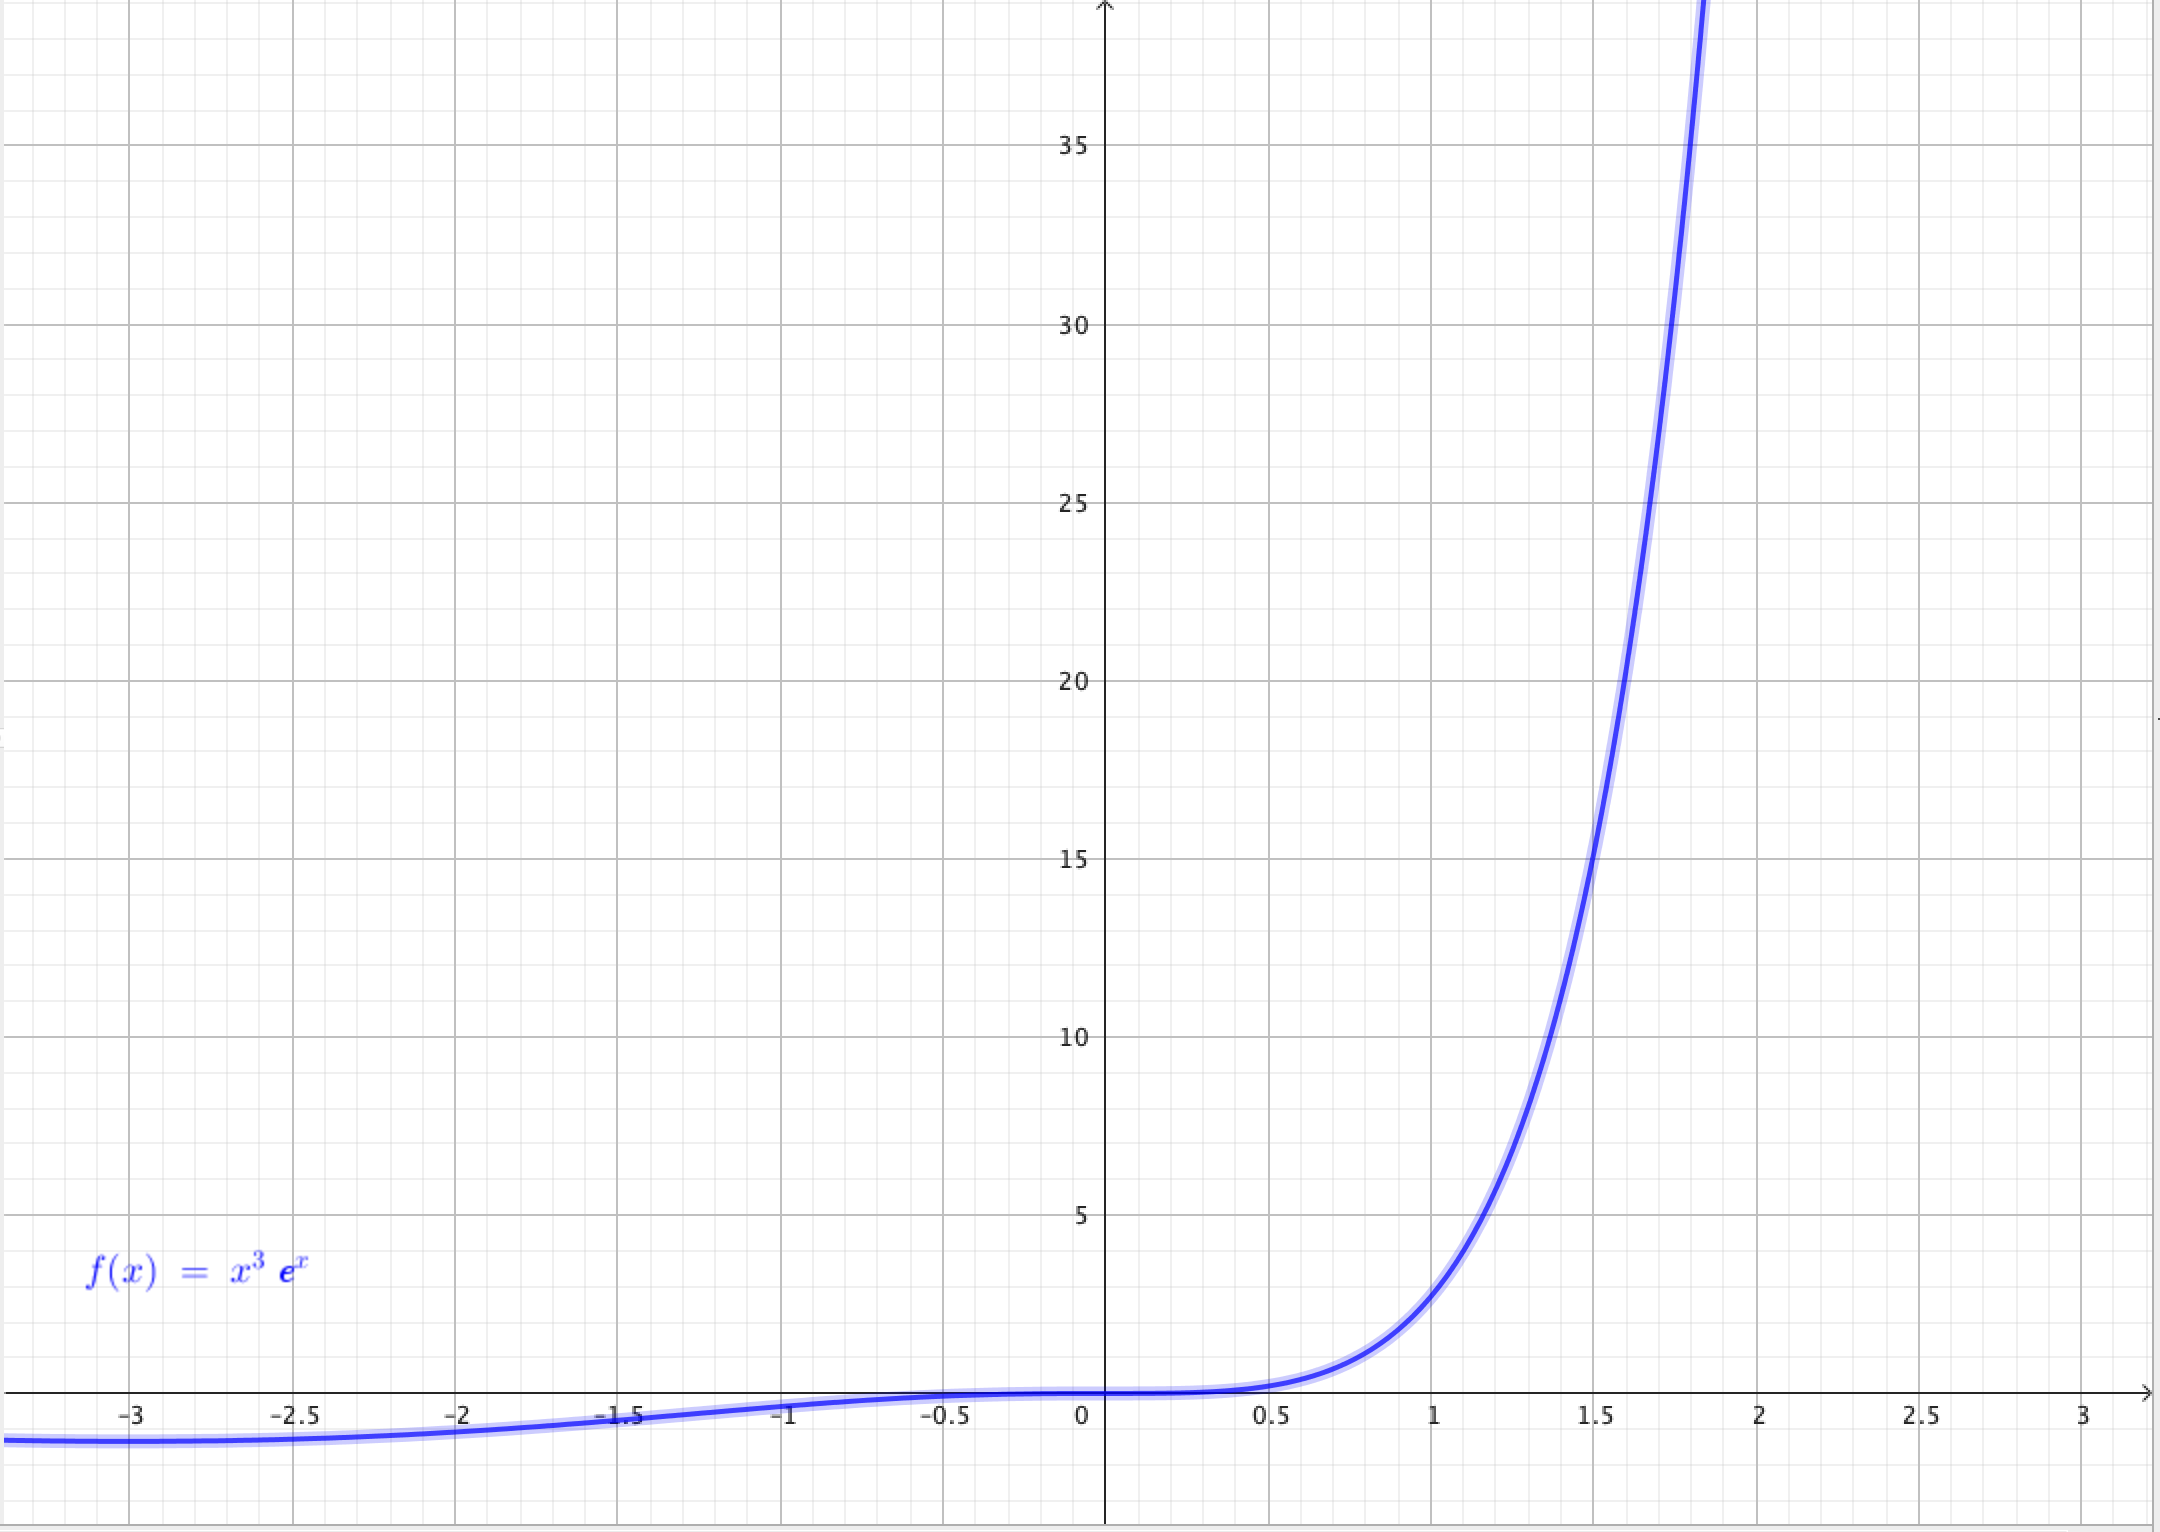
\includegraphics[scale=0.3]{Mat18_2.png}
\end{center}
\caption{Grafen for $f$ tegnet i GeoGebra}
\label{fig:2}
\end{figure}
\end{document}
